\documentclass[11pt]{article}
\usepackage[colorlinks]{hyperref}
\usepackage[margin=1in]{geometry}
\setlength{\parskip}{6pt}
\usepackage[noend]{algpseudocode}
\usepackage{enumitem}
\usepackage{graphicx}
\usepackage{wrapfig}
\usepackage{amsmath}
\usepackage{amsfonts}
\usepackage{mathtools}
\DeclareMathOperator*{\mean}{mean}
\usepackage{xspace}
\usepackage{tcolorbox}
\newcommand{\defeq}{\;\stackrel{\mbox{\tiny def}}{=}\;}
\newcommand{\horizrule}{\noindent\rule{\textwidth}{2pt}}
\newcommand{\vtheta}{\vec{\theta}}
\newcommand{\ph}{\hat{p}}
\newcommand{\ptilde}{\tilde{p}}
\newcommand{\pdisc}{p_{\rm disc}}
\newcommand{\Real}{{\mathbb R}}
\newcommand{\diffk}{\frac{\partial}{\partial \theta_k}}
\newcommand{\diffj}{\frac{\partial}{\partial \theta_j}}

\newcommand{\lesson}[1]{\href{http://cs.jhu.edu/~jason/tutorials/loglin/\##1}{lesson~#1}}
\newcommand{\Lesson}[1]{\href{http://cs.jhu.edu/~jason/tutorials/loglin/\##1}{Lesson~#1}}

\begin{document}
\title{\vspace{-2.3cm}Log-Linear Models}
\author{Jason Eisner (Johns Hopkins University)}
\date{}
\maketitle

\tcolorbox
\begin{small}
\begin{center}
This handout is intended to be used with the
    interactive visualization at
\url{http://cs.jhu.edu/~jason/tutorials/loglin/}.
\end{center}

The visualization is designed to help you understand log-linear
models, a popular and flexible family of probability distributions.
As you'll see, a conditional log-linear model defines
\begin{align*}
  p(y \mid x) & \defeq \frac{1}{Z(x)} \exp \sum_{k=1}^K \theta_k \cdot
                f_k(x,y)
\end{align*}
for some fixed set of real-valued feature functions $f_k$ with adjustable
weights $\theta_k \in \Real$.  For each $x$, the denominator $Z(x) >
0$ is a scaling factor chosen specifically
% given by
% \begin{align*}
% Z(x) & \defeq \sum_{y} \exp \sum_{k=1}^K \theta_k \cdot f_k(x,y)
% \end{align*}
% in order
to ensure that $\sum_y p(y \mid x) = 1$.

\medskip
If every $f_k$ returns values in $\{0,1\}$ only, then the above is a scaled product of
positive numbers,
\begin{align*}
p(y \mid x) & \defeq \frac{1}{Z(x)} \smashoperator[r]{\prod_{\substack{k\text{
              such that} \\ f_k(x,y)=1}}} \ \ (\exp \theta_k)
\end{align*}

Playing with the visualization will help you get the hang of
how changing the parameters $\theta_k$ affects the relative
probabilities of different $y$ values, and how those parameters can be
set automatically.  Our paper
\url{http://cs.jhu.edu/~jason/papers/#ferraro-eisner-2013} explains
why we built the visualization and what we hope you'll get out of it.
\end{small}
\endtcolorbox

\section{Starting Out Concretely}\label{sec:concrete}

\subsection{Formulas for \lesson{1}}

The four shape probabilities in \lesson{1} are computed as follows,
where $\theta_{\textrm{circle}}$ and $\theta_{\textrm{solid}}$ are the
two parameters that you can control with the sliders.  (We'll see later
in section \ref{sec:loglin} that these formulas are examples of a more
general pattern, but don't worry about that yet.)

% Note: My typesetting with \hspace here is awfully hacky.
% I should really define boxes for the summands and use the width of the boxes.

\begin{align}
p(\text{solid circle}) & \defeq \frac{\exp (\theta_{\textrm{circle}}+\theta_{\textrm{solid}})\hspace{57mm}}{\exp (\theta_{\textrm{circle}} + \theta_{\textrm{solid}}) + \exp (\theta_{\textrm{circle}}) + \exp (\theta_{\textrm{solid}}) + \exp 0} \label{eqn:solidcircle}\\
\rule{0in}{1.5\baselineskip}
p(\text{striped circle}) & \defeq \frac{\exp (\theta_{\textrm{circle}})\hspace{0mm}}{\exp (\theta_{\textrm{circle}} + \theta_{\textrm{solid}}) + \exp (\theta_{\textrm{circle}}) + \exp (\theta_{\textrm{solid}}) + \exp 0} \label{eqn:stripedcircle}\\
\rule{0in}{1.5\baselineskip}
p(\text{solid triangle}) & \defeq \frac{\hspace{44mm}\exp (\theta_{\textrm{solid}})}{\exp (\theta_{\textrm{circle}} + \theta_{\textrm{solid}}) + \exp (\theta_{\textrm{circle}}) + \exp (\theta_{\textrm{solid}}) + \exp 0} \label{eqn:solidtriangle}\\
\rule{0in}{1.5\baselineskip}
p(\text{striped triangle}) & \defeq \frac{\hspace{79mm}\exp 0}{\exp (\theta_{\textrm{circle}} + \theta_{\textrm{solid}}) + \exp (\theta_{\textrm{circle}}) + \exp (\theta_{\textrm{solid}}) + \exp 0} \label{eqn:stripedtriangle}
\end{align}

``$\exp$'' denotes the exponential function.  Recall that $\exp x$ means
$e^x$ where $e$ is a constant (namely $e=2.71828\ldots$, the base of
natural logarithms).\footnote{If $y=e^x$, then $x=\log y$.  That's the
  definition of $\log y$ (sometimes written as $\log_e y$ or $\ln y$),
  the natural logarithm.}  From the graph of $y=e^x$ you can see:

\includegraphics[height=2.25in]{exp}
\begin{minipage}[b]{4in}
\vspace{4pt}
\begin{itemize}

\item $\exp x$ is always positive (except that $\exp
  -\infty=0$).  So all of the numerators and denominators in \eqref{eqn:solidcircle}--\eqref{eqn:stripedtriangle} are
  $\geq 0$.  This makes all the probabilities $\geq 0$, as required.

\item As $x$ gets bigger, so does $\exp x$.  So raising
  $\theta_{\textrm{solid}}$ with your slider will raise the numerators
  of $p(\text{solid circle})$ \eqref{eqn:solidcircle} and $p(\text{solid triangle})$
  \eqref{eqn:solidtriangle}.  To be precise, each time you increase
  $\theta_{\textrm{solid}}$ by 1, you multiply those numerators by
  $e$.  (And decreasing $\theta_{\textrm{solid}}$ by 1 divides them by $e$.)

\item Finally, the four probabilities
  \eqref{eqn:solidcircle}--\eqref{eqn:stripedtriangle} always sum to 1
  (thanks to their common denominator $Z$).  That's required because
  those are the four possible outcomes:
\end{itemize}
\end{minipage}
\vspace{-6pt}
\begin{equation}
  p(\text{solid circle}) + p(\text{striped circle}) + p(\text{solid circle}) + p(\text{striped triangle}) = 1
\end{equation}
Hence, when raising $\theta_{\textrm{solid}}$ makes the solid
probabilities \eqref{eqn:solidcircle} and \eqref{eqn:solidtriangle} go
up, the striped probabilities \eqref{eqn:stripedcircle} and
\eqref{eqn:stripedtriangle} must go down to compensate.
This keeps the sum at 1.  Lowering $\theta_{\textrm{solid}}$ does the reverse.

\subsection{Formulas for \lesson{2}}

Now every shape has exactly two features (whereas in \lesson{1}, some shapes had fewer):

\begin{align*}
\hspace{-12mm}p(\text{solid circle}) & \defeq \frac{\exp (\theta_{\textrm{circle}}+\theta_{\textrm{solid}})\hspace{118mm}}{\exp (\theta_{\textrm{circle}} + \theta_{\textrm{solid}}) + \exp (\theta_{\textrm{circle}} + \theta_{\textrm{striped}}) + \exp (\theta_{\textrm{triangle}} + \theta_{\textrm{solid}}) + \exp (\theta_{\textrm{triangle}} + \theta_{\textrm{striped}})} \\
\rule{0in}{1.5\baselineskip}
\hspace{-12mm}p(\text{striped circle}) & \defeq \frac{\exp (\theta_{\textrm{circle}}+\theta_{\textrm{striped}})\hspace{44mm}}{\exp (\theta_{\textrm{circle}} + \theta_{\textrm{solid}}) + \exp (\theta_{\textrm{circle}} + \theta_{\textrm{striped}}) + \exp (\theta_{\textrm{triangle}} + \theta_{\textrm{solid}}) + \exp (\theta_{\textrm{triangle}} + \theta_{\textrm{striped}})} \\
\rule{0in}{1.5\baselineskip}
\hspace{-12mm}p(\text{solid triangle}) & \defeq \frac{\hspace{32mm}\exp (\theta_{\textrm{triangle}}+\theta_{\textrm{solid}})}{\exp (\theta_{\textrm{circle}} + \theta_{\textrm{solid}}) + \exp (\theta_{\textrm{circle}} + \theta_{\textrm{striped}}) + \exp (\theta_{\textrm{triangle}} + \theta_{\textrm{solid}}) + \exp (\theta_{\textrm{triangle}} + \theta_{\textrm{striped}})} \\
\rule{0in}{1.5\baselineskip}
\hspace{-12mm}p(\text{striped triangle}) & \defeq \frac{\hspace{111mm}\exp (\theta_{\textrm{triangle}}+\theta_{\textrm{striped}})}{\exp (\theta_{\textrm{circle}} + \theta_{\textrm{solid}}) + \exp (\theta_{\textrm{circle}} + \theta_{\textrm{striped}}) + \exp (\theta_{\textrm{triangle}} + \theta_{\textrm{solid}}) + \exp (\theta_{\textrm{triangle}} + \theta_{\textrm{striped}})}
\end{align*}

\section{Why We Need Log-Linear Models {\em [read after \lesson{2}]}}

{\bf Note:} Lessons 1--10 will let you experiment with simple
probabilities $p(y)$.  \Lesson{11} will finally move to the more general
case of conditional probabilities $p(y\mid x)$.  But this handout will
{\em focus} on conditional probabilities, mainly in order to avoid saying
everything twice.  If you want to think first about the case of simple
probabilities, just ignore $x$ wherever it appears; also see
section~\ref{sec:unconditioned}.

\subsection{Modeling probabilities}

We often want to model conditional probabilities like $p(y
\mid x)$, where $y$ and $x$ are discrete outcomes.
\begin{itemize}[noitemsep]
\item They can be used to predict $y$ directly, in a context $x$.
\item We can build a more complicated model as a product
  of such probabilities.\footnote{E.g., Bayes' theorem, Bayesian
    networks, (hidden) Markov models, probabilistic context-free
    grammars, \ldots}
\end{itemize}
But where do we get these probabilities?

\subsection{Notation}\label{sec:notation}

Suppose $X$ denotes a random context and $Y$ is a random event that
happens in that context.  Let $\ph(Y=y \mid X=x)$ be our estimate of
the conditional probability that the event will turn out to be $y$ when
the context happens to be $x$.  We'll abbreviate this as
$\ph(y\mid x)$.  The little ``hat'' over the $p$ is a reminder that
this is just an estimate, not the true probability.

\subsection{Simple methods}\label{sec:mle}

A simple idea is to estimate each conditional probability separately,
using simple count ratios:
\begin{equation}
\ph(y \mid x) \defeq \frac{\textrm{count}(x,y)}{\textrm{count}(x)}
\end{equation}

Such a ``maximum-likelihood'' estimate is {\em unbiased} (correct on
average, when estimated from a {\em random} dataset).  But unfortunately, it
may have {\em high variance} (it is sensitive to the {\em particular}
dataset from which you obtain the counts).  It will be unreliable if
either count is small:
\begin{itemize}[noitemsep]
\item Suppose the denominator $\textrm{count}(x)$ is 2, then the estimate
  will be either 0, 0.5, or 1.  These estimates are quite different,
  and which one you get depends on your particular dataset.
\item It's even worse if the denominator is 1 or 0.  What happens in
  each case?
\item If the numerator $\textrm{count}(x,y)$ is 0, meaning that $y$
  was not {\em observed} in context $x$, then the estimate will
  be 0, jumping to the conclusion that $y$ is essentially {\em impossible} in context $x$.
\item If the numerator is 1, then the estimate might be too high,
  since perhaps $y$ is just one of many unlikely events---it's the one
  we happened to see.
\end{itemize}

\noindent
``Smoothing'' techniques try to reduce the variance of this estimate.
However, they still estimate each conditional probability more or less
independently of the others.\footnote{Though ``backoff smoothing'' does jointly
  estimate $p(y \mid x_1)$ and $p(y \mid x_2)$ if $x_1, x_2$ are
  related in a certain way.}
% so that $\ph(y \mid x_1) \approx \ph(y \mid x_2)$ if the contexts
% $x_1 \approx x_2$ are similar and have small counts,
%  but not in a very flexible way.

\section{Log-Linear Models {\em [read after \lesson{2}]}}\label{sec:loglin}

Log-linear modeling is a very popular and flexible technique for
addressing this problem.  It has the advantage that it considers {\em
  descriptions} of the events.  Contextualized events $(x,y)$ with
{\em similar descriptions} tend to have {\em similar probabilities}---a form
of generalization.
% That is, if $\vec{f}(x_1,y_1) \approx \vec{f}(x_2,y_2)$, then
% $\hat{p}(y_1 \mid x_1) \approx \hat{p}(y_2 \mid x_2)$.

\subsection{Feature functions}\label{sec:featfuncs}

Since you are the one who knows something about your problem, {\em
  you} get to define the function $\vec{f}$ that extracts these
descriptions.  If you decide that your model will have $K$ features,
then $\vec{f}(x,y)$ denotes a vector of $K$ real numbers $(f_1(x,y),
f_2(x,y), \ldots, f_K(x,y))$ that {\em describe} event $y$ in context
$x$.  These $K$ numbers are called the {\bf values} or {\bf strengths}
of the features.

\medskip

You might use the following set of 5 features ($K=5$) to describe
colored shapes against backgrounds.  The third column gives the
feature values for a dark striped circle $y$ against a light
background $x$:

\smallskip\noindent
\begin{tabular}{|c|l|c|} \hline
feature number & feature meaning   & feature value on this example \\ \hline
1              & $y$ is circular   &    1 \\
2              & $y$ is square     &    0 \\
3              & $y$ is striped    &    1 \\
4              & $y$ is a striped square & 0 \\
5              & how strongly $y$ contrasts with background $x$ & 2 \\ \hline
\end{tabular}
\smallskip

\noindent Thus, your description of this particular $(x,y)$ is given by
$\vec{f}(x,y)=(1,0,1,0,2) \in \Real^5$.  In English, you can say
that features 1, 3, and 5 {\bf fire} on this contextualized event
$(x,y)$, and that feature 5 fires twice (or fires with strength 2).

% That means that you chose to describe the contextualized event $(x,y)$
% as ``having'' features 1, 3, and 5 but not features 2 and 4.
%
% Furthermore, by defining $f_5(x,y)=2.0$, you chose to say that $(x,y)$
% has feature 5 especially strongly.  A common figure of speech is that
% feature 5 {\bf fires} especially strongly on $(x,y)$.

\medskip
It is slightly unusual that $f_5(x,y)=2.0$.  In principle a feature
value $f_k(x,y)$ can be any positive or negative real number.  But
most often your feature functions $f_k$ will be boolean functions, so
that $f_k(x,y)$ is always either 1 or 0, according to whether $(x,y)$
has feature $k$ or not.

% \subsection{Scores}


\subsection{The defining formula}\label{sec:formula}

% !!! perhaps define score.
% And perhaps define set of outcomes Y for each x:
%    see discussion at https://piazza.com/class/hzdzwofeqmh54o?cid=63 .

The log-linear probability model computes a contextualized
event's probability from its features.
% CHANGED THIS BACK - WE NOW USE \hat{\theta} but not \ph
% \footnote{We are still using the
%   $\ph$ notation because this is only a model that we are trying to
%   fit to the data.  In most cases, we will never know whether the true
%   probability distribution $p$ has this form.}
For example, given a
light background $x$, how likely is the shape $y$ to be a dark striped circle?

Specifically, the log-linear model defines
\begin{equation}\label{eqn:loglin}
  p(y \mid x) \defeq \frac{\ptilde(x,y)}{Z(x)}
\end{equation}
where the interesting part is the {\bf unnormalized probability}
defined by
\begin{align}\label{eqn:unnorm}
  \ptilde(x,y) &\defeq \exp \sum_{k=1}^K \left( \theta_k \cdot f_k(x,y) \right)  \\
         &= \exp \left(\vtheta \cdot \vec{f}(x,y)\right) > 0
\end{align}
Here $\vtheta \in \Real^K$ is a vector of feature {\bf weights}, which
are the adjustable parameters of the model.  You control these
with sliders in the interactive visualization.  

\medskip
The unnormalized probabilities $\ptilde(x,y)$ are always positive (because
of the $\exp$).  Equation~(\ref{eqn:loglin}) has to scale them, in
order to get proper probabilities that sum to 1 (i.e., $\sum_y
p(y\mid x) = 1$ for each $x$).  As you can see in
(\ref{eqn:loglin}), this is a simple matter of dividing them by a {\bf
  normalizing constant}, namely

\vspace{-16pt}
\begin{equation}
  Z(x) \defeq \sum_y \ptilde(x,y)
\end{equation}

Note that the conditional log-linear modeling framework has allowed us
to model $p(y \mid x)$ directly, rather than as a quotient $p(x,y) /
p(x)$.  We did not have to commit to any model of $p(x)$.

\subsection{Feature weights}

You can easily see that for any choice of $\vtheta$ and any $x$,
equation~(\ref{eqn:loglin}) gives a genuine probability distribution
over the events $y$ that could occur in context $x$.  You can also see
now why the model is ``log-linear''---for each context $x$, the
log-probability is a linear function of the feature vector:
\begin{equation}\label{eqn:logversion}
\log p(y \mid x) = \vtheta \cdot \vec{f}(x,y) - \log Z(x)
\end{equation}

% LEAVE THIS FOR THE ONLINE LESSONS
% This doesn't mean that our model $p$ is the {\em correct}
% distribution!  Does $p(y \mid x)$ equal the true probability?
% There is no guarantee that the true probability can be accurately
% described at all using a log-linear model with these features,
% let alone with the specific weights $\vtheta$.

In our earlier example, setting the parameter $\theta_5 > 0$ makes
contrasting colors more common: the resulting $p(y \mid x)$ says
that dark shapes $y$ are probable when the background $x$ is light,
and vice-versa.  Alternatively, setting $\theta_5 < 0$ makes
contrasting colors less common.

\medskip
In general, the linear coefficients $\vtheta$ in \eqref{eqn:logversion} are incredibly
important: the way you pick them will determine all the probabilities
in the model, and even the normalizing constants!  Fortunately, to
help you set $\vtheta$, you'll have a training set of events in their
contexts, $\{(x_1,y_1), (x_2,y_2), \ldots (x_N,y_N)\}$.  Then the
weight vector $\vtheta$ that maximizes
\begin{equation}\label{eqn:loglin-likelihood}
\prod_{i=1}^N p(y_i \mid x_i)
\end{equation}
does the best possible job of predicting these events in their
contexts.  More on this later.

\subsection{Unconditioned Models}\label{sec:unconditioned}

The initial lessons in the interactive visualization deal with the
simple case where there is no information about context.  So we can
omit $x$.  We now have a simple distribution over possible $y$ values,\looseness=-1

\vspace{-16pt}
\begin{align}
  p(y) &\defeq \frac{\ptilde(y)}{Z} \label{eqn:unconditioned} \\
  \ptilde(y) &\defeq \exp \left(\vtheta \cdot \vec{f}(y)\right) > 0 \\
  Z &\defeq \sum_y \ptilde(y)
\end{align}
\vspace{-12pt}

For example, in the first two lessons, \eqref{eqn:unconditioned} is
used to define two probability models over the four shapes
$y \in {\cal Y} = \{\text{solid circle}, \text{striped circle},
\text{solid triangle}, \text{striped triangle}\}$.
Look back at section~\ref{sec:concrete} of this
handout to see the concrete formulas for the probabilities of the 4
shapes, which sum to 1.

\medskip
In each of these models, a shape's features are computed by
functions like $f_{\textrm{solid}}(y)$, which returns 1 on the solid
circle and solid triangle, and returns 0 on the other two shapes.
Therefore, the parameters of the model are feature weights like
$\theta_{\textrm{solid}} \in \Real$.  The larger $\theta_{\textrm{solid}}$ is,
the more the probability distribution favors the solid circle and
solid triangle.

\subsection{Features versus Attributes}

In practical settings, the outcome $y$ and the context $x$ are
characterized by their {\em attributes} (or {\em properties}).  Each
feature's value is then computed from one or more of these attributes.
$f_4$ and $f_5$ from section~\ref{sec:featfuncs} would be defined more
formally as
\begin{align}
f_4(x,y) & \defeq (\textsc{fill}(y)=\text{striped}) \wedge (\textsc{shape}(y)=\text{square})
             & \text{\small\it ``$y$ is a striped square''} \\
f_5(x,y) & \defeq |\textsc{brightness}(y)-\textsc{brightness}(x)|/100
             & \text{\small\it ``how strongly $y$ contrasts with background $x$''}
\end{align}
which refer to the \textsc{fill}, \textsc{shape}, and \textsc{brightness} attributes
of $y$ and/or $x$.

\medskip
You will sometimes hear people refer to individual attributes as the
``features'' or ``basic features'' of $x$ and $y$.  That's confusing.
I recommend that you use ``features'' only to refer to feature
functions (like $f_4$) or to the feature values that they return (like $f_4(x,y)$).

\subsection{Remark: Named Features and Efficient Dot Products}

In the notation above, we assigned numbers $1,2,\ldots,K$ to the
features.  This lets you represent the parameter vector $\vtheta$
(as well as each feature vector $\vec{f}(x,y)$) by an {\em array} of
$K$ real numbers.

\medskip
However, it is often more convenient to refer to the features by names
instead of numbers.  The names can be strings or other objects that
describe the feature.  For example, in the table from
section~\ref{sec:featfuncs}, the first feature function might be
called $f_{\sf circle}$ instead of $f_1$, with corresponding weight
$\theta_{\textsf{circle}}$ instead of $\theta_1$.  Then the weight vector
$\vtheta$ can be implemented as a hash table instead of an array.  It
still maps the index $k$ to the weight $\theta_k$, but now $k$ is a
name instead of a number.

\medskip
The dot product $\vtheta \cdot \vec{f}(x,y)$ is now defined by
$\sum_k \theta_k \cdot f_k(x,y)$ where $k$ ranges over the set of
feature names.
In computing this sum, it is fine to skip features $k$ where $f_k(x,y)
= 0$.  In many cases, this is a big speedup because only a few of the
$K$ features will fire on a given contextualized event $(x,y)$.  For
example, $f_k(x,y)$ will be 1 for only one of the shapes $k \in \{{\sf
  circle}, {\sf square}, \ldots\}$, and 0 for all other shapes.  So the
sum includes just one of the weights $\theta_{\textsf{circle}},
\theta_{\textsf{square}}, \ldots$.

\medskip
In our example from section~\ref{sec:featfuncs}, $\vtheta \cdot \vec{f}(x,y)$ could be efficiently
computed as
\begin{algorithmic}
\State $s \gets 0$\Comment{initialize sum}
\State $s \gets s + \theta_{\textrm{shape}(y)}$\Comment{add weight of
  the single binary shape feature that fires on $y$: e.g.,
  $\theta_{\textsf{circle}}$}
\If{$y$ is striped}
  \State $s \gets s + \theta_{\textsf{striped}}$
  \If{$y$ is square}
    \State $s \gets s + \theta_{\textsf{striped square}}$
  \EndIf
\EndIf
\State $s \gets s + \theta_{\textsf{contrast}} \cdot f_{\textsf{contrast}}(x,y)
$\Comment{where $f_{\textsf{contrast}}(x,y) \equiv ||\textrm{color}(x)-\textrm{color}(y)||$
  is not binary}
\end{algorithmic}

\subsection{Remark: Other names for log-linear models}

Log-linear models $p(y)$ and conditional log-linear models
$p(y\mid x)$ are so prevalent that they have been rediscovered many
times!  So you will see lots of names for them.  The following are all
roughly equivalent: log-linear models, Gibbs distributions, undirected
graphical models, Markov Random Fields or Conditional Random Fields,
exponential models, and (regularized) maximum entropy models.
Special cases include logistic regression and Boltzmann machines.

\medskip
In all these cases, you define a probability by multiplying some
positive numbers together and dividing by a constant $Z$ so that your
probabilities will sum to 1.

\section{Finding the Parameters {\em [read with \lesson{6}]}}

We will try some examples in the interactive visualization where it's
tricky to adjust $\vtheta$ by hand.  So let's ask, how {\em should}
one adjust it?

\subsection{An intuition}

It turns out that maximizing equation (\ref{eqn:loglin-likelihood}) is
not too hard.  Suppose your training set has $N=100$ events of which
80 are circles (some solid, some striped).  But your current $\vtheta$
says that circles only happen 0.7 of the time, i.e.,
$$p(\textrm{striped circle}) + p(\textrm{solid circle}) = 0.7$$
so your model predicts that only 70 of the 100 events should be circles.
%
In that case, you should increase the weight of the ``circle''feature,
because the {\bf expected count} $70$ is smaller than the {\bf
  observed count} $80$ ($E < O$) and so you need to make circles more
likely in your model.  Similarly, if $E > O$ then you should decrease this weight.
Either way, by gradually adjusting this weight you can make $E=O$, so
that your model correctly predicts the observed number of circles.

\medskip
As you've probably noticed, the feature weights do interact.  Once
you've made $E=O$ for the circle feature, trying to make $E=O$ for the
striped feature may mess up your first move, so that $E \neq O$ again
for the circle feature.  However, if you keep gradually adjusting all
of the features in this way, either simultaneously or one at a time,
then you will eventually reach a setting where $E=O$ for all features!

\subsection{The justification}

The setting where $E=O$ for all features is actually the
setting of $\vtheta$ that maximizes equation
(\ref{eqn:loglin-likelihood}), or equivalently, the setting that
maximizes the logarithm of (\ref{eqn:loglin-likelihood}):\footnote{It
  just happens that the logarithm is easier to work with
  mathematically, because of the $\exp$ in (\ref{eqn:unnorm}).  But
  why is it equivalent to maximize the logarithm?  Because $p_1 > p_2$
  if and only if $\log p_1 > \log p_2$.  That is, $\log p$ is
  an increasing function of $p$ (look at the graph of the $\log$ function).%
  % , which implies that
  % increasing $p$ will also increase $\log p$.  So if we are not yet at
  % a maximum of $p$, then we should be able to increase $p$ and
  % therefore we are still able to increase $\log p$.  Only when $\log
  % p$ reaches a maximum is $p$ maximized.
}
\begin{align}
  F(\vtheta) & \defeq \log \prod_{i=1}^N p(y_i \mid x_i) = \sum_{i=1}^N \log p(y_i \mid x_i)
\label{eqn:loglin-log-likelihood}
\end{align}

\subsection{Formula for the gradient}

You can see this by computing the partial derivatives of $F(\vtheta)$
with respect to the $k$ weights:

\begin{align}
  \diffk F(\vtheta)
  &= \sum_{i=1}^N \diffk \log p(y_i \mid x_i)  \\ %   - \left( \theta_k / \sigma^2 \right)
  &= \sum_{i=1}^N \diffk \log \ptilde(y_i \mid x_i) - \diffk \log Z(x_i) \\
  & \hspace{1in}\vdots \nonumber \\
  &= \underbrace{\left( \sum_{i=1}^N f_k(x_i,y_i) \right)}_{\textit{observed count $O_k$ of feature $k$}}
  - \underbrace{\left( \sum_{i=1}^N \sum_y p(y\mid x_i) f_k(x_i,y) \right)}_{\textit{expected count $E_k$ of feature $k$}} \label{eqn:obsexp}
\end{align}

At the max of $F(\vtheta)$, this derivative must be 0 for each
$\theta_k$, and hence $E_k=O_k$ for each feature $k$.

\medskip
{\bf Clarification:} So far in the online toy, you have only been
modeling $p(y)$.  However, soon you'll try $p(y\mid x)$ as
defined in section~\ref{sec:formula}.  What does ``expected count'' mean in this
setting?  (\ref{eqn:obsexp}) defined it as $\sum_{i=1}^N \sum_y
p(y\mid x_i) f_k(x_i,y)$.  This counts how many times $f_k$ would
have fired on average if we had still observed exactly the same
training contexts $x_1,\ldots x_n$, but if the corresponding training events
$y_1,\ldots y_n$ were respectively replaced by random draws from the
conditional distributions $p(y \mid x_i)$.

\subsection{Algorithm for maximizing the log-probability}\label{sec:concave-claim}

It can be shown that $F$ is a concave function (see Appendix~\ref{app:hessian}), so it is like a simple hill with only one local maximum.  There are many reasonable ways to climb to the top of this hill.  One option is {\bf gradient ascent},\footnote{\label{fn:sgd}For large $N$, it is popular nowadays to use
  {\bf stochastic gradient ascent}, which is faster in practice because it does not have to fully evaluate the sum $F(\vtheta) = \sum_{i=1}^N \cdots$ or $\diffk F(\vtheta) = \sum_{i=1}^N \cdots$ before updating $\vtheta$.  Rather, it updates to improve each summand in turn.  \href{http://research.microsoft.com/pubs/192769/tricks-2012.pdf}{Bottou (2012)} gives a good presentation with practical advice.} a
simple function maximization algorithm that increases $\theta_k$ at a
rate proportional to $\diffk F(\vtheta)=O_k-E_k$, for all $k$ in parallel.
These partial derivatives are positive when $E_k < O_k$ or negative
when $E_k > O_k$.  In the interactive visualization, they will be displayed
as ``hints'' on the sliders if you check the ``Show gradient'' box (see \lesson{6}).
You can see that as you adjust the $\vtheta$ sliders, these partial derivatives 
also gradually change---eventually reaching 0 at the top of the hill, where
$E_k=O_k$ exactly for all $k$.

The final value of $\vtheta$---at the top of the hill---is our estimate of the ``true'' 
$\vtheta$ value that we have assumed to exist.  (It might sometimes be
denoted by $\widehat{\vtheta}$, since a ``hat'' indicates an estimate
(as in section~\ref{sec:notation}).  The true value would be denoted
by $\vtheta^*$.)

\subsection{Detailed derivation for the curious}\label{sec:bias-claim}

We got to (\ref{eqn:obsexp}) above by applying basic rules
of differentiation:
\begin{align}
  \diffk \log \ptilde(y \mid x)
  &= \diffk \left( \sum_{k=1}^K \theta_k \cdot f_k(x,y) \right) \\
  & = \diffk \left( \theta_k \cdot f_k(x,y) + \textrm{constant not involving $\theta_k$} \right) = f_k(x,y)\\
%
  \diffk \log Z(x) &= \frac{1}{Z(x)} \diffk Z(x)
  = \frac{1}{Z(x)} \sum_y \diffk \ptilde(x,y)  \\
  &= \frac{1}{Z(x)} \sum_y \diffk \exp (\vtheta \cdot \vec{f}(x,y))\\
  &= \frac{1}{Z(x)} \sum_y \left( \exp (\vtheta \cdot \vec{f}(x,y)) \right)
  \left( \diffk (\vtheta \cdot \vec{f}(x,y)) \right) \\
  &= \frac{1}{Z(x)} \sum_y \ptilde(x,y) \cdot f_k(x,y) \\
  &= \underbrace{\sum_y p(y\mid x) \cdot f_k(x,y)}_{\textit{expected value $e_k(x)$ of feature $k$ in context $x$}} \label{eqn:exp}
\intertext{hence}
  \diffk \log p(y \mid x) 
  &= \diffk \log \ptilde(y \mid x) - \diffk \log Z(x) = f_k(x,y) - e_k(x) \label{eqn:obsexp-deriv}
\end{align}

Equation~\eqref{eqn:obsexp} simply sums this over all training pairs $(x_i,y_i)$ to 
find that $\diffk F(\vtheta) = \sum_i f_k(x_i,y_i) - e_k(x_i)$.

\emph{Cool remark:} The function $-\frac{1}{N} F(\vtheta)$ gives the average surprisal of a training example.  Differentiating with respect to $\theta_k$, we get $\mean_i e_k(x_i) - f_k(x_i,y_i)$.  This can be regarded as the model's \emph{bias}---its average error in predicting feature $k$ when using the current parameters.  And Appendix~\ref{app:hessian} shows that differentiating twice with respect to $\theta_j$ and $\theta_k$, we get the \emph{covariance} of the model's predictions of features $j$ and $k$!

\section{Regularizing the Parameter Estimates {\em [read with \lesson{8}]}}\label{sec:regularization}

Problems sometimes arise when we simply maximize the log-probability.
Why does this happen?  Can we fix it?

\subsection{Overfitting, underfitting, and the bias/variance tradeoff}

You saw in \lesson{8} that maximizing $F(\vtheta)$ might actually be a
bad idea.  The resulting estimate of $\vtheta$ makes the {\em
  training} data very probable, but it might not generalize well to
{\em test} data.  That is called {\bf overfitting} the training data.

In fact, there is a close connection to the bad unsmoothed estimates
of section~\ref{sec:mle}, which also overfitted.  Both cases use {\bf
  maximum-likelihood estimates}---that is, they model the training
data as well as they can, using the available
parameters.\footnote{Technically, the {\bf likelihood} of the
  parameter vector $\vtheta$ is defined by
  (\ref{eqn:loglin-likelihood}), which says how probable the training
  data would be if we used {\em that} $\vtheta$.  We have been finding
  the {\bf maximum-likelihood} estimate of $\vtheta$ by maximizing the
  likelihood (\ref{eqn:loglin-likelihood}) or equivalently the
  log-likelihood (\ref{eqn:loglin-log-likelihood}).}

\subsection{How many parameters?}

What are the available parameters?  In section~\ref{sec:mle} we were
able to choose the probabilities individually, so we could model the
training data perfectly (a bad idea!).  But now we can only manipulate
the probabilities indirectly through the $\vtheta$ parameters of our
log-linear model.

If the log-linear model has only a few parameters, that may save us
from overfitting---we will be unable to fit the training data too
closely, which forces us to generalize.  You saw this in \lesson{3} of
the interactive visualization.  On the other hand, if the log-linear
model has enough features, as in \lesson{4}, then you can again fit the
training data perfectly.  Maximizing (\ref{eqn:loglin-likelihood})
will then get you exactly the same bad probabilities as in
section~\ref{sec:mle}.

So perhaps we should simply build a simple log-linear model with few
parameters.  But wait \ldots do we really want to break our good model
and get rid of potentially useful features??  Then we might have a
problem of {\bf underfitting}---not matching the training data closely
enough.

In general, it's reasonable for the number of parameters to increase
with the size of the training data.  We see exactly the same issue
when choosing between bigram and trigram models.  We should be able to
match true English better with a trigram model (or better yet, a
50-gram model), but we may not have enough training data to estimate
trigram probabilities accurately.  In that case we fall back to a
bigram model, which reduces variance (to avoid overfitting) but
unfortunately increases bias (leading to underfitting).

\subsection{The regularization idea}

We'd prefer not to make a strict choice between pure bigram and
pure trigram models.  The training corpus may have plentiful evidence
about {\em some} trigrams while lacking evidence about others.  This
line of thinking leads to backoff smoothing---the topic of the next
assignment.

How does this idea apply to log-linear models?  In general, we'd like
to include a whole lot of potentially useful features in our model,
but use only the ones that we can estimate accurately on our
particular training data.  Statisticians call this idea {\bf
  regularization}.  In the log-linear setting, a feature with weight 0
has no effect on the model, and a feature with low weight has little
effect.  So the regularization principle is ``All weights should stay
close to 0, except where really needed to model the data.''

So instead of maximizing the log-likelihood
(\ref{eqn:loglin-log-likelihood}), let's maximize the
{\bf regularized log-likelihood},
\begin{equation}\label{eqn:loglin-regularized}
  F(\vtheta) = \left( \sum_{i=1}^N \log p(y_i \mid x_i) \right) - C\cdot R(\vtheta)
\end{equation}
where $R(\vtheta)$ is a penalty for weights that get far away from 0.
A parameter $C \geq 0$, which can be tuned via cross-validation, will control the size of this penalty and
hence the strength of regularization.

\subsection{Types of regularization}

A common choice is called $\ell_2$ (or $L_2$) regularization.  Define
$R(\vtheta) = ||\vtheta||^2 = \sum_i \theta_i^2$.  Then
\begin{equation}
  \diffk F(\vtheta) = \textrm{observed count of $k$} -
  \textrm{expected count of $k$} \underbrace{\mbox{}-2C \cdot
    \theta_k}_{\textit{new term}}
\end{equation}
Because of the new term, gradient ascent will tend to push $\theta_k$
toward 0 (increase it if it's negative, decrease it if it's positive).
For large values of $C$, the optimal $\theta_k$ will be usually be
close to 0.  {\em However,} if feature $k$ is sufficiently common in the
training data, then $\diffk F(\vtheta)$ will be dominated by the
counts, and the regularization term will have comparatively little
influence.  In this case, $\theta_k$ will be able to pull farther away
from 0 in order to model the observations---which is exactly what we
wanted to happen for well-observed features.

Another common choice is $\ell_1$ (or $L_1$) regularization.  Here
$R(\vtheta) = \sum_i |\theta_i|$.  Then
\begin{equation}
  \diffk F(\vtheta) = \textrm{observed count of $k$} -
  \textrm{expected count of $k$} \underbrace{\mbox{}-C\cdot \textrm{sign}(\theta_k)}_{\textit{new term}}
\end{equation}
This has a similar effect.  See Appendix~\ref{app:more-regularization} for the differences.

Notice that for any $C > 0$, regularization will always prevent
$\theta_k$ from zooming off to $\infty$ or $-\infty$ (because that
would make $R(\vtheta)$ infinitely bad).  Happily, this prevents us from
estimating $p(y\mid x)=0$ as happened in \lesson{8}.

With either $\ell_2$ or $\ell_1$, the function $F(\vtheta)$ in \eqref{eqn:loglin-regularized} is concave---in fact strictly concave.\footnote{Why? Because $F(\vtheta)$ is a sum of concave functions.  We noted earlier that log-likelihood is a concave function (see Appendix~\ref{sec:hessian} for a proof).  The regularizer $R(\vtheta)$, it is a strictly convex function, which becomes strictly concave when we ``turn it upside down'' by multiplying it by $-C < 0$.  Their sum is therefore strictly concave.} So it has a single global maximum that can be found efficiently by greedily climbing the hill.

\appendix
\clearpage
\section{More Remarks on Regularization {\em [read if curious]}}\label{app:more-regularization}

\subsection{Which regularizer to use?}

%%%%%%%%%%%%%%%%%%%%%%%%%
% L1-L2.png was created like this in gnuplot:
%
% # set termoption dash   # allow dashed lines
% set term pngcairo dashed   # make PNG file, and allow dashed lines
% set output "L1-L2.png"
% set key bottom left
% l(x) = -0.05*(x*2+3)**2-1
% plot [-1.2:1.2] l(x) title "log likelihood" linewidth 2 linecolor rgb "blue", -abs(x) title "L1 (with C=1)" linewidth 2 linecolor rgb "red" linetype 1, -x**2 title "L2 (with C=1)" linewidth 2 linecolor rgb "green" linetype 1, l(x)-abs(x) title "log likelihood + L1" linecolor rgb "red" linetype 2, l(x)-x**2 title "log likelihood + L2" linecolor rgb "green" linetype 2
%%%%%%%%%%%%%%%%%%%%%%%%%

Optimization is relatively easy with $\ell_2$ because the regularizer
is differentiable.  This lets you use standard optimization techniques
that rely on the gradient (e.g., L-BFGS or stochastic gradient ascent).

\paragraph{Advantage of $\ell_1$:  Sparse solutions.}  The main reason to consider $\ell_1$ instead is that it is a ``sparsity-inducing regularizer.''  As we saw in \lesson{9}, the optimal $\vtheta$ will tend to be a {\em sparse vector} with many zero elements, especially if $C$ is large.

You may prefer to have many zero elements: you won't need to compute $f_k(x,y)$ at test time if $\theta_k=0$.  So this regularizer does {\bf feature selection} for you: it identifies a small set of useful features that deserve to get nonzero weights.  The resulting model may be easier for you to interpret, and is small and fast at test time.

Why does $\ell_1$ regularization have this effect?  This graph shows a particular parameter $\theta_k$ on the $x$ axis.  Suppose that $\theta_k=0$.  We could increase the log-likelihood by decreasing $\theta_k$.  However, this wouldn't help the log-likelihood (blue curve) as much as it would hurt the regularizer (red curve)!  We therefore prefer to keep $\theta_k$ at 0, to avoid decreasing the {\em total} function $F(\vtheta)$ (dashed red curve).

\begin{wrapfigure}{r}{3in}
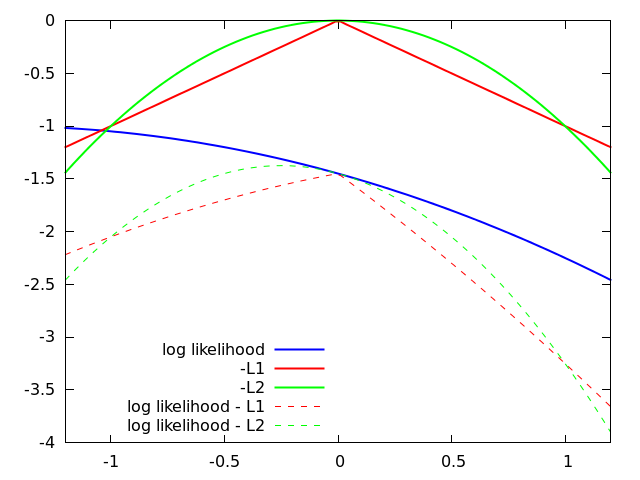
\includegraphics[width=3in]{L1-L2}
\end{wrapfigure}

In general, moving $\theta_k$ away from 0 {\em in either direction} will increase the $\ell_1$ regularization penalty at rate $C$ (where $C=1$ in this drawing).  Hence we will not be willing to do this unless it increases the log-likelihood at an even greater rate, that is, $|\diffk F(\vtheta)| > C$.  That's not the case in the situation shown.

An $\ell_2$ regularizer does {\em not} promote sparsity.  If $\theta_k=0$, we can again increase log-likelihood (blue curve) by decreasing $\theta_k$---but this time, we may as well do so, since the regularizer (green curve) has a flat derivative at $\theta_k=0$ and so will suffer only negligible harm if we move a tiny bit leftward.  Notice that the total function $F(\theta)$ (dashed green curve) is differentiable and happens to have its maximum at $\theta_k < 0$. Once we use $\ell_2$, there is nothing very special about 0 anymore---it would be surprising if the maximum were achieved at $\theta_k=0$ exactly.

\paragraph{Computational disadvantage of $\ell_1$: More complicated optimization.}
We already mentioned that with either $\ell_2$ or $\ell_1$, the objective function is concave.
However, with $\ell_1$, it is somewhat harder to perform the maximization.  The practical difficulty is that $F(\vtheta)$ (dashed red line) is non-differentiable, so methods like gradient ascent and L-BFGS no longer work.\footnote{The simplest approach is the {\bf subgradient method}.  However, this is not very good at achieving sparsity: even when the optimum $\vtheta$ is sparse, so that some elements of $\vtheta$ will converge to 0 {\em in the limit}, these elements may never hit 0 exactly {\em in finite time}.  A popular approach that fixes this is the {\bf proximal gradient} algorithm, which is explained along with other approaches in the monograph of \href{http://www.di.ens.fr/~fbach/bach_jenatton_mairal_obozinski_FOT.pdf}{Bach et al. (2012)}.  {\bf Stochastic gradient ascent} (footnote \ref{fn:sgd}) can also be adapted to this setting, as explained by \href{http://www.aclweb.org/anthology/P09-1054}{Tsuruoka et al. (2009)} and \href{http://www.jmlr.org/papers/volume12/shalev-shwartz11a/shalev-shwartz11a.pdf}{Shalev-Shwartz and Tewari (2011)}.}

\paragraph{Statistical disadvantage of $\ell_1$ (and of sparsity in general): Forced choices.}\label{sec:eggs}
Consider the setting where you have two features that fire in very similar circumstances on training data: $f_1(x,y) \approx f_2(x,y)$.  In that case, which feature should get
the higher weight?  Consider 3 of the options that must be chosen among when maximizing \eqref{eqn:loglin-regularized}:
\begin{itemize}[noitemsep]
\item $\theta_1=b,\ \theta_2=b$  (for some constant $b$)
\item $\theta_1=2b,\ \theta_2=0$
\item $\theta_1=0,\ \theta_2=2b$
\end{itemize}
In all three cases, the model will assign pretty much the same
probabilities, since $\vtheta \cdot \vec{f}(x,y)$ is not changed when
we shift weight between the similar features $f_1$ and $f_2$.  So it
is the regularizer (not the log-likelihood) that will make the choice.

The $\ell_2$ regularizer prefers the first option, which divides the weight evenly between the two features.  (That's because $b^2+b^2$ is smaller than $(2b)^2+0^2$ or $0^2+(2b)^2$.)  Thus, it doesn't commit to one feature over the other.  Both features will be considered equally at test time.

The $\ell_1$ regularizer thinks all three of these cases are {\em equally} good.  (That's because $b+b = 2b+0 = 0+2b$.)  In practice, however, real numbers are rarely {\em exactly} equal.  Since the features $f_1$ and $f_2$ are not {\em quite} identical, something will break the tie.  The choice will probably be more like this:
\begin{itemize}[noitemsep]
\item $\theta_1=1.5,\ \theta_2=1.7$  (for some constant $b$)
\item $\theta_1=0,\ \theta_2=3.4$
\item $\theta_1=3.0,\ \theta_2=0$
\end{itemize}
and in this case, the $\ell_1$ regularizer will prefer the third option (since it wants to minimize $|\theta_1|+|\theta_2|$).  This shouldn't be surprising since $\ell_1$ likes a sparse weight vector.  However, $\ell_1$ is putting all its eggs in one basket (as any feature selection method does).  It ``arbitrarily'' selects $f_1$ as important and $f_2$ as irrelevant, even though they had very similar behavior on training data.  It might turn out that this was the wrong decision.  Perhaps $f_2$ is actually more helpful for this problem in general, even though $f_1$ appeared to be slightly more helpful on the limited sample of training data.

\paragraph{Why $\ell_1$ and not $\ell_0$?}  If your goal is to achieve sparsity, then $\ell_1$ is not quite appropriate.  You should really use $\ell_0$, where $\ell_0(\vtheta)$ returns the number of nonzero elements of $\vtheta$.  Keeping this small is equivalent to keeping the vector sparse.  If you really think that only a few features are relevant, then $\ell_0$ assesses whether your weight vector is plausible.  However, using $\ell_0$ would make $F(\vtheta)$ really hard to maximize.  So $\ell_1$ is commonly used as a convex approximation to $\ell_0$.\footnote{What would it take to maximize exactly using $\ell_0$ regularization?  Notice that it is straightforward to maximize the log-likelihood {\em after} you have done feature selection.  For example, you can find the values of $\theta_2, \theta_5, \theta_7$ that are optimal when you require all other weights to be 0.  (The $\ell_0$ regularizer would be pretty happy with this $\vtheta$, since $R(\vtheta)=3$ is nice and small, but the log-likelihood may not be so great since your model only has 3 features.)  You could repeat this convex maximization for {\em each} subset of the $K$ features, and return the model for which the regularized log-likelihood \eqref{eqn:loglin-regularized} is maximized.  Unfortunately, this method involves looping over all $2^K$ subsets!
  %
  An approximate version is called {\bf forward selection}.  Instead of trying all $2^K$ subsets, greedily expand the feature set by one feature at a time
  (starting with the empty set), in a way that increases \eqref{eqn:loglin-regularized} as fast as possible until it can't be increased anymore.  This no longer takes exponential time, but it is still rather slow.}

In fact, what you want is probably $\ell_0 + \ell_2$, which says ``Try to have a small set of nonzero weights, and keep those small.''  A common choice is to approximate this by $\ell_1+\ell_2$ (the ``elastic net'' regularizer), giving a concave $F(\vtheta)$.  Note that when you add two regularization terms in this way, you probably want to give them separate coefficients (both tuned on dev data).  A nice trick is to optimize with $\ell_1+\ell_2$ to accomplish feature selection, and then remove the weight-0 features and re-optimize the other weights with $\ell_2$ only (``debiasing'').


\subsection{A interpretation of regularization as MAP estimation}

One way to interpret regularization is in terms of Bayes'
Theorem.  Suppose we want to find the most likely value of $\vtheta$,
given the training data.  That is, instead of choosing $\vtheta$ to
maximize $p(\textrm{data} \mid \vtheta)$ (the {\bf maximum likelihood}
principle), we'll more sensibly choose it to maximize $p(\vtheta \mid
\textrm{data})$ (the {\bf maximum a posteriori (MAP)} principle).  By
Bayes' Theorem, $p(\vtheta \mid \textrm{data})$ is proportional to
\begin{equation}
\underbrace{p(\textrm{data} \mid \vtheta)}_{\textit{likelihood}} \cdot \underbrace{p(\vtheta)}_{\textit{prior}}
\end{equation}
And maximizing the log of this is precisely the same as maximizing
(\ref{eqn:loglin-regularized}), provided that we define $p(\vtheta)$
to be proportional to $\exp -R(\vtheta)$.  In other words, our prior
distribution says that if $R(\vtheta)$ is large then $\vtheta$ has low
probability.  From this point of view, $\ell_2$ regularization
corresponds to a Gaussian prior,\footnote{Since the exp of a quadratic
  function is a Gaussian function.  This looks like a bell curve in
  $k$ dimensions, with most of the probability near the
  origin: \includegraphics[scale=0.4]{gaussian} This choice explicitly defines the prior
  probability of $\vtheta$ to be proportional to $\exp -\frac{1}{2\sigma^2} \sum_k
  \theta_k^2$, where $\sigma^2 (= 1/2C)$ is called the {\em variance} of the
  Gaussian.  Clearly, this is just a convenient assumption about
  where the true value of $\vtheta$ is most likely to fall.%
  % (Similarly, add-$\lambda$ smoothing (even with backoff) can be
  % derived from a certain prior assumption about the true probabilities
  % $p(z \mid xy)$.  Ask me if you're curious.)
}  and $\ell_1$
regularization corresponds to an exponential prior.  Both of these say
that {\em a priori}, we expect each $\theta_k$ to be close to 0.

\subsection{The full Bayesian treatment}

MAP estimation as in the previous section is sometimes called {\bf empirical Bayes}.  But a real Bayesian wouldn't just use the single best choice of $\vtheta$.  After all, Bayes' Theorem doesn't pick one $\vtheta$ for us; it gives us a whole posterior probability distribution over models, $p(\vtheta \mid \textrm{data})$.  This represents our uncertainty about what the true $\vtheta$ is.  So ideally, we would average over all of these models, like this!
\begin{align}
\ph(y \mid x)
&= \int_{\vtheta\in \Real^K} p(y, \vtheta \mid x)\,d\vtheta \\
&= \int_{\vtheta\in \Real^K} p(y \mid x,\vtheta)\cdot p(\vtheta \mid \textrm{data}) \,d\vtheta
\end{align}
where $p(y \mid x,\vtheta)$ is the conditional distribution given by a log-linear model with parameters $\vtheta$.

This {\bf fully Bayesian} approach gives a principled solution to our feature selection dificulty from section \ref{sec:eggs}.  Suppose you have a Bayesian prior that explicitly prefers a sparse solution, for example $\exp -R(\theta)$ where $R$ is the $\ell_0+\ell_2$ regularizer.  Then the $\vtheta$ vectors that are most probable ({\em a posteriori} as well as {\em a priori}) will generally be sparse.  But since we're not sure which one is correct, we average over their predictions.  We are no longer choosing just one sparse vector from which to make our predictions; that is, we no longer put all our eggs in one basket.

The fully Bayesian approach to log-linear models is the ``right way''
to use them.  Unfortunately, it is highly computationally intensive.
There is some work on it, but it is not widely used in practice.

\section{Second derivatives  {\em [read if curious]}}\label{app:hessian}

Recall equation~\eqref{eqn:obsexp-deriv}:
$$\diffk \log p(y \mid x) = f_k(x,y) - e_k(x)$$

You can differentiate this a second time to get the second derivative $\diffj
\diffk \log p(y \mid x)$, which also turns out to have a nice form:
\begin{align}
  \diffj \diffk \log p(y \mid x) &= -\underbrace{\sum_{y'} p(y' \mid x) \left( f_j(x,y') - e_j(x) \right)
                                   \cdot \left( f_k(x,y') - e_k(x)
                                   \right)}_{\textit{covariance of
                                   features $j$ and $k$ in context
                                   $x$}} \label{eqn:covar}
\end{align}
where $e_j(x)$ and $e_k(x)$ are defined by \eqref{eqn:exp}.  Isn't that cute?

Equation~\eqref{eqn:covar} is the negated covariance of $f_j(x,y')$
and $f_k(x,y')$ when $y'$ is randomly distributed (given $x$)
according to the model.  Note that it does not depend on $y$.

The Hessian of $\log p(y \mid x)$ is therefore a negated covariance
matrix, which means that it must be negative semidefinite.  And since
$F(\vtheta) = \sum_i \log p(y_i \mid x_i)$, its Hessian is a sum of
such matrices, so it is also negative semidefinite.  This proves the
claim in section~\ref{sec:concave-claim} that $F(\vec{\theta})$ is
concave.

Alternatively, the Hessian of $-\frac{1}{N}F(\vtheta)$ can also be
regarded directly as a covariance matrix, specifically the covariance
matrix of $\vec{f}(x,y)$ when $x$ is distributed according to the
dataset and $y$ given $x$ is distributed according to the model.  This
means that $-\frac{1}{N}F(\vtheta)$ must be convex, again proving that
$F(\vec{\theta})$ is concave.  As noted in
section~\ref{sec:bias-claim}, the function $-\frac{1}{N}F(\vtheta)$
can be interpreted as ``average surprisal'' and its gradient can be
regarded as a bias vector, which goes nicely with the observation that
its Hessian can be regarded as a covariance matrix.

\subsection{Detailed derivation for the \emph{really} curious}

We can check that equation~\eqref{eqn:covar} is correct:
\begin{align}
 & -\sum_{y'} p(y' \mid x) \left( f_j(x,y') - e_j(x) \right) \cdot \left( f_k(x,y') - e_k(x) \right) \\
 &= - \sum_{y'} p(y' \mid x) \underbrace{\left( f_j(x,y') - e_j(x)
   \right)}_{\textit{see \eqref{eqn:obsexp-deriv}}} \cdot f_k(x,y')
   \nonumber \\
 &\quad  + \underbrace{\left( \sum_{y'} p(y' \mid x) \left( f_j(x,y') - e_j(x) \right) \right)}_{\textit{$= 0$ by definition of $e_j(x)$}} \cdot e_k(x) \label{eqn:zeroexp}\\
 &= - \sum_{y'} p(y' \mid x) \underbrace{\left( \diffj \log p(y' \mid
   x) \right)}_{\textit{differentiate by chain rule}} \cdot f_k(x,y')
   = - \sum_{y'} p(y' \mid x) \frac{1}{p(y' \mid x)} \diffj p(y' \mid
   x) \cdot f_k(x,y') 
   \raisetag{12pt} \label{eqn:logderivative} \\
 &= - \sum_{y'} \left( \diffj p(y' \mid x) \right) \cdot f_k(x,y') \text{ where each $f_k(x,y')$ is a constant}\\
 &= - \diffj \underbrace{\sum_{y'} \left( p(y' \mid x) \cdot
   f_k(x,y')) \right)}_{\textit{see \eqref{eqn:exp}}} \text{ i.e., the derivative of a linear combination} \\
 &= - \diffj e_k(x) 
   \quad = \diffj\underbrace{(f_k(x,y) - e_k(x))}_{\textit{see
   \eqref{eqn:obsexp-deriv} again}} \text{ for any $y$, since $f_k(x,y)$ is a constant} \\
 &= \diffj \diffk \log p(y \mid x) 
\end{align}

Step~\eqref{eqn:zeroexp} notes that the difference of $f_j$
from its expectation is 0 on average---that's in the nature of an
expectation.  You could write this out formally
as $\sum_{y'} p(y' \mid x) \left( f_j(x,y') - e_j(x) \right) =
\left( \sum_{y'} p(y' \mid x) f_j(x,y') \right) - \left( \sum_{y'}
  p(y' \mid x) \right) \cdot e_j(x) = e_j(x) - 1 \cdot e_j(x) = 0$.

% Alternative treatments are in notes by
% \href{http://qwone.com/~jason/writing/convexLR.pdf}{Jason Rennie} or
% \href{http://www.cs.cmu.edu/~nasmith/papers/smith.tut04.pdf}{Noah
% A. Smith}.

\end{document}
